\chapter{Contribuição: StarVZ sobre Spark} \label{ch:contribution}

A fase de pré-processamento do arcabouço StarVZ é similar a um fluxo de Ciência 
de dados. Nele, são carregadas e manipuladas várias tabelas, utilizando 
bibliotecas do pacote \texttt{tidyverse}. Este Capítulo fala sobre as diferenças 
propostas e realizadas no StarVZ, com o objetivo de otimizar o tempo de 
execução desta fase. Resumidamente, no lugar de tabelas R, utilizaremos tabelas
Spark (\emph{Spark Dataframes}) para o carregamento e manipulação de dados.
Na Seção \ref{sect:arch} são apresentadas as mudanças 
arquiteturais propostas e na Seção \ref{sect:implement}, detalha-se a 
implementação dessas mudanças.

\section{Arquitetura Proposta} \label{sect:arch}

A arquitetura da aplicação que este trabalho se propõe a modificar pode ser visualizada na Figura \ref{fig:starvz-app}.
Os dados, já em formato CSV são lidos com a biblioteca \texttt{readr}. Com estes em memória, são realizadas filtragens e junções com
o auxílio das bibliotecas \texttt{dplyr} e \texttt{tibble}. Finalmente, os dados são escritos em disco no formato \texttt{Feather}, 
usando a biblioteca de mesmo nome. Todo esse processo é conduzido através de um código R.

\begin{figure}[ht]
 \centerline{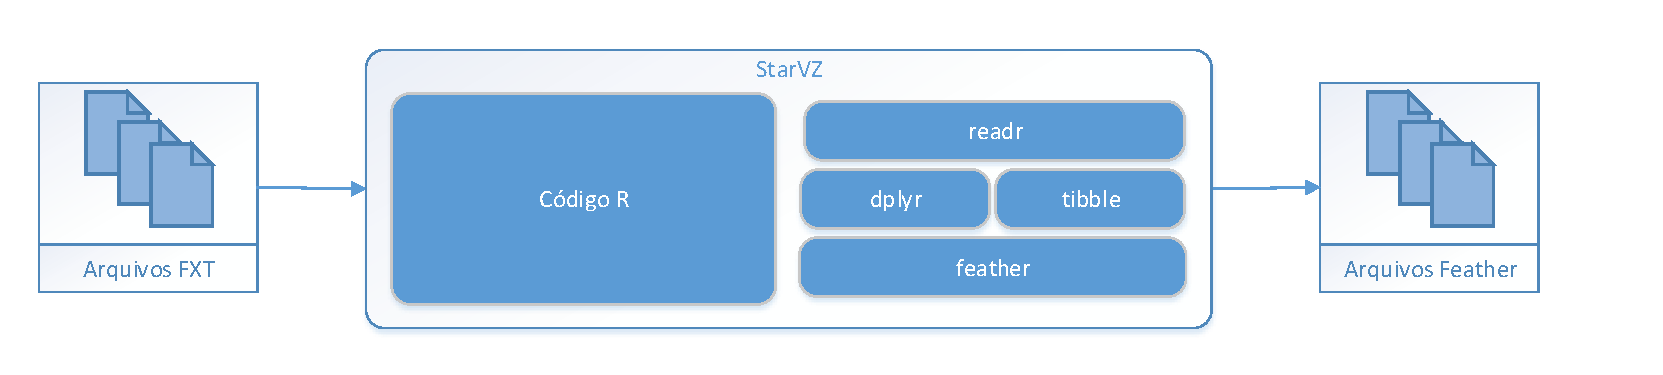
\includegraphics[width=1\textwidth]{./img/starvz-arch.pdf}}
 \caption{Arquitetura da aplicação StarVZ.}
 \label{fig:starvz-app}
\end{figure}

Durante o trabalho, identificou-se que não havia uma biblioteca que suportasse a escrita de tabelas Spark em arquivos \texttt{Feather}.
Isso é essencial para compararmos a escrita do mesmo tipo de dados tanto na execução sequencial quanto na distribuída utilizando tabelas Spark.
Devido ao ecossistema Hadoop utilizar o formato \texttt{Parquet} \cite{} como padrão para armazenamento de dados colunares, a aplicação 
foi adaptada para escrever suas saídas neste formato. Isso foi realizado utilizando a biblioteca Apache arrow \cite{}, a arquitetura final da aplicação sequencial pode ser visualizada na Figura \ref{fig:starvz-app-arrow}. 

\begin{figure}[ht]
 \centerline{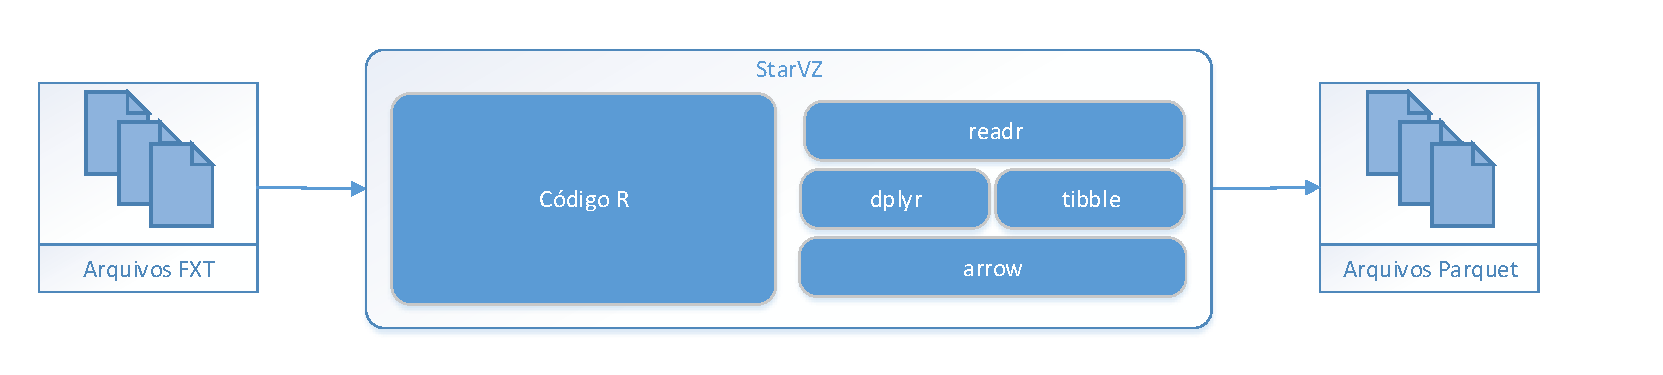
\includegraphics[width=1\textwidth]{./img/starvz-arch-arrow.pdf}}
 \caption{Arquitetura da aplicação StarVZ adaptada para escrever Parquet.}
 \label{fig:starvz-app-arrow}
\end{figure}

A Figura \ref{fig:starvz-app-spark} ilustra a arquitetura da aplicação após as modificações propostas. Considerando o tamanho dos arquivos de entrada, utilizaremos o HDFS para armazená-lo. Todavia, alguns arquivos não crescem muito com o aumento do tamanho das entradas, ficando com o tamanho na ordem de KBytes. Para esses arquivos pequenos, o custo de armazená-los no sistema de arquivos e tratá-los no 
sistema de arquivos distribuído é maior do que armazená-los e trata-los sequencialmente e, por isso, seu armazenamento e tratamento continuou no formato sequencial. A escrita das saídas foi padronizada para escrever com o sparklyr no HDFS, dessa forma o usuário 
tem apenas uma fonte de saída.

\begin{figure}[ht]
 \centerline{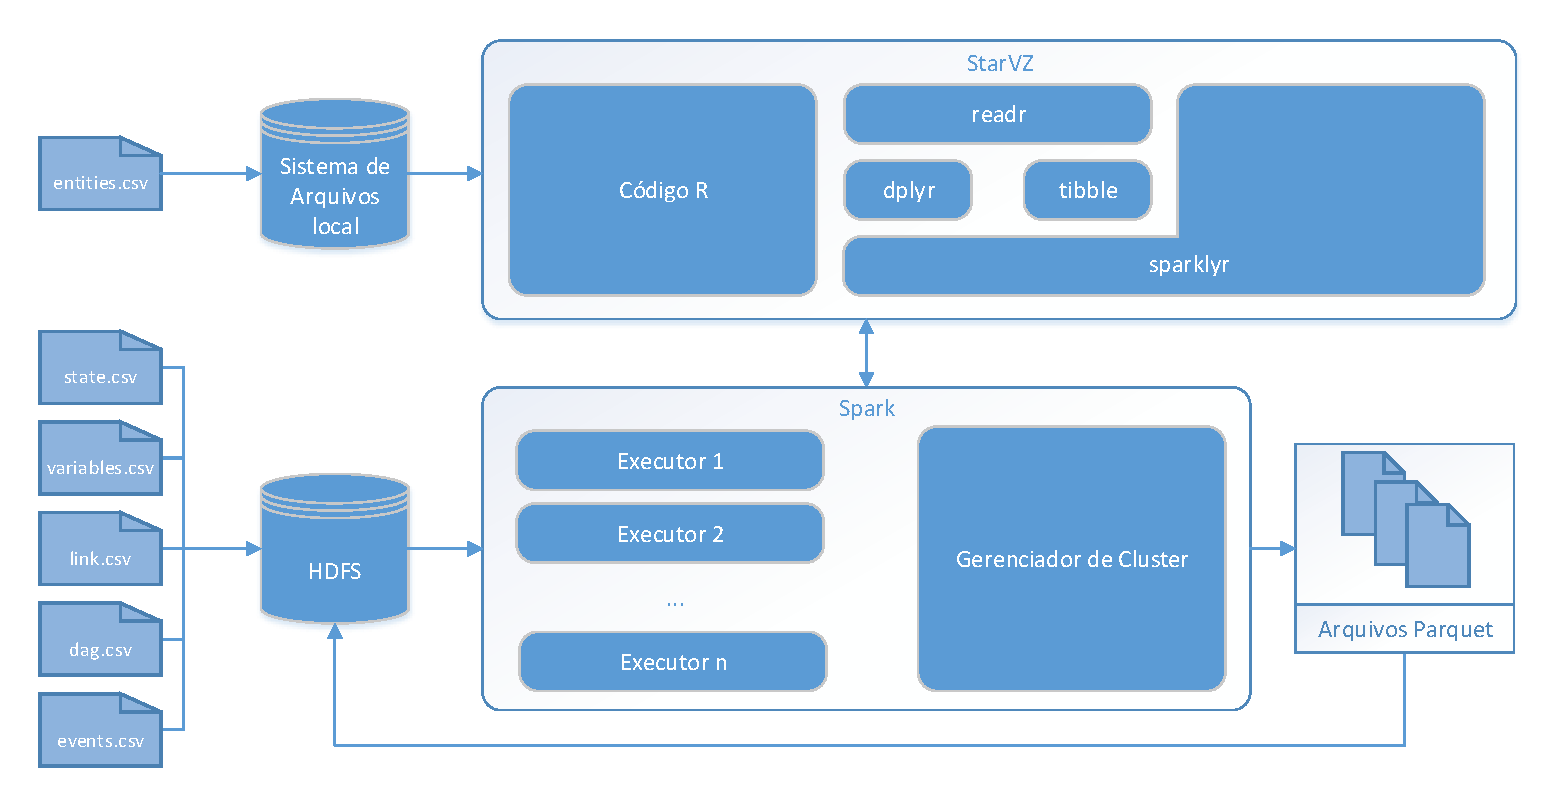
\includegraphics[width=1\textwidth]{./img/starvz-arch-spark.pdf}}
 \caption{Arquitetura da aplicação StarVZ utilizando Spark.}
 \label{fig:starvz-app-spark}
\end{figure}

\section{Implementação} \label{sect:implement}

Tratando-se dos detalhes de implementação, foi criado um novo arquivo com o fluxo de dados distribuído.
Dessa forma, em um único pacote, o usuário pode optar por realizar a execução sequencial ou distribuída do arcabouço.
Criou-se o parâmetro de execução de tipo, onde \texttt{-S} significa sequencial e \texttt{-D} significa distribuída.

Na parte sequencial, a escrita de arquivos foi modificada para ser realizada com o pacote arrow. Em termos de código, essa
modificação é bastante pontual, adicionando uma importação de biblioteca e modificando-se os métodos de escrita de arquivos
(de \texttt{write\_feather} para \texttt{write\_parquet}). É importante salientar que este pacote também possui uma implementação
de \texttt{write\_feather}, que é mais eficiente que aquela do pacote \texttt{feather}. Além disso, começamos a medir o tempo de
execução em diversos pontos, que serão aprofundadados no Capítulo \ref{ch:evaluation}.

A execução distribuída precisou uma expansão nos parâmetros para comportar o diretório no HDFS, o \texttt{gerenciador de cluster} 
no qual o spark irá buscar recursos e o local de instalação do spark. Isso flexibiliza a aplicação, já que o usuário pode executar 
em diferentes gerenciadores de cluster (por exemplo, executar em um gerenciador local com cargas de trabalho pequenas e distríbuido
com cargas de trabalho maiores, apenas mudando um parâmetro). A informação de diretório de entradas locais também é necessária, 
tendo em vista que alguns arquivos não compensam ser carregados do HDFS e tratados de forma distribuída.

A biblioteca \texttt{sparklyr} fornece uma forma de interação com tabelas R praticamente igual a \texttt{dplyr}, o que 
facilitou bastante a adaptação. De acordo com \citet{}, a abordagem dessa biblioteca difere da abordagem padrão das APIs 